\section{Itération 0}

\subsection{Présentation du contexte}

Dans le cadre de notre Licence Fondamentale en Sciences de L'informatique à 
la Faculté des Sciences de Sfax,Nous avons utilisé nos connaissances pour 
réaliser un projet de fin d'études pendant un stage dans Djagora Academy .
Ce chapitre présente une mise en contexte et une description de la problématique
et trace les objectifs de notre projet.De tel projet consiste a réaliser une
plateforme
Avant de commencer la première itération du Scrum, une période de temps à été
consacrée pour préparer ce qui est nécessaire au lancement du projet dans de bonnes
conditions. cette période est souvent nommé l’itération 0 du projet. Elle est consacrée
généralement à la recherche bibliographique, aux choix technologiques et à la mise en
place de l’environnement de développement. Outre que ces préparatifs, c’est dans cette
itération que nous définissons le Backlog de la Plateforme, ainsi que le nombre
d’itérations nécessaires et la durée de l’itération. Il s’agit aussi d’une période de
formation pour les membres de l’équipe sur tous les environnements et les technologie à
utiliser au cours du montage du produit.

\subsection{Présentation de l'Académie}

Djagora Academy est un programme dont l'objectif est la mise en pratique des
aspects philosophiques liés au Leadership et à l'Entrepreneurship.

Il est à noter que le Leadership ou/et l'entrepreneurship inefficace/s
demeure/ent un obstacle majeur aux actions industrielles, économiques,
humanitaires, etc., efficaces.
Basé sur la méthodologie dite «le Leadership Diamond®», développée par Dr. Peter
Koestenbaum et présentée à la Faculté des Sciences de Sfax Dr. Mahamouda
Salouhou\footnote{visiter think.factorycampus.net pour plus de détails},
L'académie Djagora est vue comme un programme de mentorat visant accompagner des
étudiants (mentorés) en année terminale par des universitaires et des
industriels (mentors) avec le soutien de plusieurs compagnies internationales,
telles que l'European Center for Leadership and Entrepreneurship Education
(Eclee France, Eclee USA), Djagora University (SénégaL), NorthStar Paradigm
Education (USA), Continental (Allemagne), Sivantos (Allemagne), Yousoft-IT
(Tunisie), Factory Campus (Tunisie) dans la réalisation de projets d’intérêt
publique.

%Considérés comme des idées de startups, les projets proposés par le comité de
%pilotage de l'Académie Djagora se substituent aux projets de fin d'études.
%La durée de réalisation d’un projet s’étale sur cinq mois. Cette période
%correspond à un cycle d’accélération de startups. Tout au long de ce cycle,
%les mentorés suivront un programme de formations généralement certifiantes.

Mis-à-part le programme de mentorat et le cycle d’accélération de startups,
l'Académie Djagora déclare le défi et organise une compétition tout au long
du cycle d’accélération de startups. Nommée «Bourse des startups», cette
compétition unique en son genre, dont l'idée est attribuée à Factory Campus,
est une bonne opportunité pour tous les intervenants de l'Académie Djagora.
La «Bourse des startups» vise joindre l'utile du modèle financier et des retombées
économiques de la bourse et de l'entrepreneuriat en général à l'agréable des
bonnes pratiques et cultures du défi, de la concurrence, du challenge et du
leadership.

\subsection{Présentation du sujet}

 Le projet consiste en la création d'un système logiciel de collecte, 
 de traitement, d'analyse, de fouille et de visualisation des données/informations.
 Il est décomposé en deux sous systèmes. L'un se charge de la collecte. L'autre,
 quant à lui, est chargé du reste; du traitement à la visualisation. 
 Celui, chargé de la collecte, peut être assimilé dans un premier temps 
 à une application mobile capable de collecter des informations. Dans ce cas, 
 l'information est collectée soit d'une façon automatique en se basant uniquement 
 sur les capteurs intégrés aux smartphones/tablettes (mobile sensors), 
 soit encore de façon semi-automatique faisant appel aux simples intéractions 
 de l'utilisateur (utilisateur citoyen). Le deuxième sous système peut être 
 assimilé à une application web permettant le traitement, l'analyse syntaxique
 et sémantique, la fouille des informations/données collectées (big data et
 data-mining) pour enfin assurer leur visualisation. \\
En prenant départ d'un récepteur de position, le sujet mit à résoudre les
problématiques localisations de multiple individu,la réalisation d'un module
d'itinéraire pour les véhicules vers enfin la création d'un mécanisme qui donne
la main à effectuer divers types de rapport dans une carte.

La figure~\ref{fig:citywatch-architecture} représente le flux des informations
géographiques dés l'envoye des coordonnées depuis les satellites GPS aux smartphones
dans les véhicules, les informations sont ensoite envoyées au serveur à travers
le réseaux cellulaire et l'internet pour les analyser et les stocker. A la fin,
elles seront accessibles par le tableau du board de CityWatch.

\begin{figure}[htbp]
  \centering
  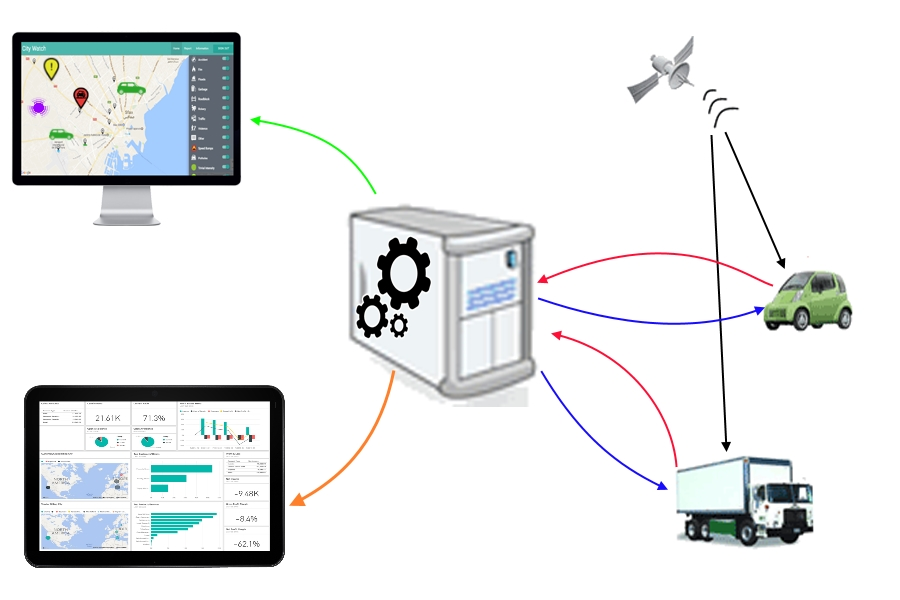
\includegraphics[width=0.8\textwidth]{citywatch-architecture}
  \caption[Flux des information Géographiques en CityWatch]
  {Flux des informations Géographiques dans le systéme de tracking de la plateforme CityWatch}
  \label{fig:citywatch-architecture}
\end{figure}

\subsection{Méthode de gestion de projet utilisée}

\subsubsection{Présentation de la méthode agile SCRUM}

Scrum est une méthode de gestion de projets dans laquelle des équipes
multifonctionnelles réalisent des produits de manière itérative et incrémentale. Tout au
long de cette méthode, le développement est définit, d’une façon incrémentale, en cycles
de travail appelés Sprints. Un sprint est définit sous la forme d’un certain nombre de
tâches à réaliser au cours d’une itération. Cette dernière ne dure jamais plus que quatre
semaines (deux semaines la plupart du temps). Les itérations s’enchainent l’une après
l’autre sans interruption. Les Sprints se terminent à une date spécifique. Ceux-ci ne
peuvent être prolongés même si le travail ne soit pas terminé. Généralement les équipes
Scrum choisissent une durée de Sprint et la maintiennent durant le projet, jusqu’à ce
qu’elles puissent encore augmenter leur productivité et utiliser alors un cycle plus court.
Au début de chaque Sprint, une équipe multifonctionnelle (environ de quatre à sept
personnes) sélectionne des tâches (exigences du client) dans une liste priorisée.
L’équipe s’accorde collectivement sur une cible constituée de ce qu’elle pense pouvoir
livrer à la fin du Sprint. Aucune nouvelle tâche n’est ajoutée durant le Sprint. Chaque
jour, l’équipe se réunit brièvement afin de contrôler sa progression et ajuster les
prochaines étapes nécessaires à la finalisation du travail restant au sein d’un Sprint. A la
fin de chaque Sprint, une revue est organisée avec les parties prenantes durant laquelle
l’équipe montre ce qu’elle a réalisé. Le feedback obtenu peut être pris en compte sur le
Sprint suivant. Scrum insiste sur la nécessité de livrer un produit opérationnel,
testé et documenté à la fin de chaque itération.
la figure~\ref{fig:scrum-model} représente la méthode agile SCRUM.

%\documentclass{standalone}

%\usepackage{mathpazo}
%\usepackage{tikz}

\usetikzlibrary{calc}
\usetikzlibrary{positioning}
\usetikzlibrary{shapes}

%\begin{document}

\tikzstyle{box} = [rectangle, rounded corners, draw=black, text width=10em, minimum height=3em, text centered]
\begin{figure}[htbp]
  \centering
  \footnotesize
  %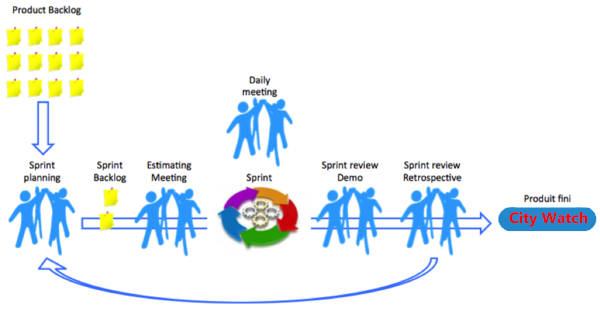
\includegraphics[width=\textwidth]{./figures/scrum-model.tex}
\begin{tikzpicture}

  \node[box]
    (sprints) {Sprints};
  \node[box, left=4em of sprints]
    (planning) {Planning \& System Architecture};
  \node[box, right=4em of sprints]
    (closure) {Closure};

  \draw[->,latex-,line width=0.1em] (5:6em) arc (5:85:6em) node[right=2em] {Wrap};
  \draw[->,latex-,line width=0.1em] (95:6em) node[left=2.5em] {Develop} arc (95:175:6em);
  \draw[->,latex-,line width=0.1em] (185:6em) arc (185:265:6em) node[left=2em] {Adjust};
  \draw[->,latex-,line width=0.1em] (275:6em) node[right=2.5em] {Review} arc (275:355:6em);

  \draw[->,latex-] (planning.west) -- +(-2em,0);
  \draw[->,-latex] (planning.east) to (sprints.west);
  \draw[->,-latex] (sprints.east) to (closure.west);
  \draw[->,-latex] (closure.east) -- +(2em,0);

\end{tikzpicture}
\caption[Méthode Scrum]{La méthode Génie Logiciel Scrum comme décrite par \textcite{Schwaber1995}.}
\captionsource{Daniel G. Siegel, Typical Development Processes of Free and Open Source Software Projects}
\label{fig:scrum-model}
\end{figure}

%\end{document}


\paragraph{Pourquoi Scrum?}

Scrum place l’humain au centre de la méthodologie. Le client intervient tout au long
du processus de création et l’équipe travaille en collaboration, et aussi parce que cette
méthode est idéale pour le cas d’une petite équipe et le fait d’avoir un grand projet réparti
entre cette équipe.
L’application de Scrum m’a permis de raccourcir les délais de production et d’avoir
un produit final qui correspond au plus près aux besoins du client.

\subsubsection{Répartition des rôles}

Chaque projet utilisant la méthode Scrum est monté autour d’une équipe auto-
organisée et multifonctionnelle : auto-organisée car il n’y a pas de chef d’équipe qui
décide les rôles de chacun, ou de la manière dont un problème est résolu, puisque ces
problématiques sont traitées par l’équipe dans son ensemble; et multifonctionnelle car
chaque membre de l’équipe forme une partie prenante dans le développement de
chaque fonctionnalité depuis l’idée jusqu’à l’implémentation finale.
Dans Scrum existe trois principaux rôles:
\begin{itemize}
 \item Le responsable produit (Product owner)
 \item Le Scrum Master
 \item le membre de l’équipe
\end{itemize}

\paragraph{Le responsable produit}

Il prend en charge de communiquer la
vision globale du produit à l’équipe.
Il se voit représenter le client final, se met à sa place
et priorise ses besoins. Celui qui tient ce rôle est celui qui
a le plus de visibilité, de responsabilité et d’autorité.
En effet, la méthode Scrum favorise l’auto-organisation de l'équipe.

\paragraph{Le Scrum Master}

Il joue le rôle du communiquant entre le responsable produit et
l’équipe. Il ne gère pas l’équipe, mais veille à éliminer tous les obstacles qui peuvent
empêcher l’équipe d’atteindre les objectifs fixés au cours d’un Sprint. En résumé, ce rôle
permet à l’équipe de rester créative et productive, tout en veillant à ce que les
réalisations soient visibles pour le responsable produit.

\paragraph{L'équipe}

Dans la méthode Scrum, l’équipe est responsable de la réalisation
opérationnelle des Sprints. L’équipe est généralement composée de personnes
multitâches. C’est toute l’équipe qui est responsable du résultat final de chaque sprint.
La manière dont sont exécutées les tâches est très libre mais cette liberté doit être
néanmoins cadrée par l’obligation de répondre aux objectifs du sprint.

\subsubsection{Durées estimées}

Pour montrer l’avancement durant une itération donnée, on a besoin de tracer le
Burndown Chart. Il s’agit d’un graphique simple qui montre le nombre d’heures restant
à effectuer pour finaliser le produit.

\subsubsection{Modélisation UML}

\subsection{Backlog générale}

La première étape de la méthode Scrum consiste à préparer un carnet du produit
(Product Backlog) qui présente la liste des tâches à effectuer durant le développement
du projet qui sera répartie en des itérations. Le rôle du product-owner est important
dans cette phase de développement parce qu’il devra faire l’exercice de prioriser ses
demandes selon des critères respectant la mission et les objectifs de son produit. En
précisant la valeur de priorité, il estime l’impact et le retour sur investissement 
qu’aura chacun des items dans le carnet du produit.
Il y a donc effectivement eu un gros travail
d’échanges et discussions avec le client pour comprendre tout le cahier des charge
initial,C’est comme ça que le Backlog a été défini.

La figure~\ref{fig:product-backlog} présente une version simplifié du product
backlog décrit dans le tableau~\ref{tab:product-backlog}.
%\usepackage{dtklogos}
\usetikzlibrary{mindmap,shadows}
% Information boxes
\newcommand*{\info}[4][16.3]{%
  \node [ annotation, #3, scale=0.65, text width = #1em,
          inner sep = 2mm ] at (#2) {%
  \list{$\bullet$}{\topsep=0pt\itemsep=0pt\parsep=0pt
    \parskip=0pt\labelwidth=8pt\leftmargin=8pt
    \itemindent=0pt\labelsep=2pt}%
    #4
  \endlist
  };
}
\begin{tikzpicture}[every annotation/.style={draw, fill=white, font=\Large}]
    \renewcommand{\href}[2]{#2}

    \path[mindmap,
          concept color=black!40,
          text=white,
          every node/.style={
              concept,
              circular drop shadow,
              execute at begin node=\hskip0pt,
          },
          %grow cyclic,
          root/.style={
              concept color=black!40,
              fill=white, line width=1ex, text=black,
              font=\footnotesize\bfseries,
              text width=7em},
          level 1 concept/.append style={
              font=\normalsize\bfseries,
              sibling angle=50,
              text width=7.7em,
              level distance=12.5em,
              inner sep=0pt},
          level 2 concept/.append style={
              font=\footnotesize\bfseries,
              level distance=8em},
    ]

    node[root] {Platforme CityWatch} [clockwise from=0]
    child[concept color=blue!60] {
        node {Gestions des Rapports} [clockwise from=90]
        child { node (goForum) { Consultation } }
        child { node (goWiki) { Déclaration } }
    }
    child[concept color=blue] {
        node[concept] {Systeme de protection }
        [clockwise from=30]
        child { node[concept] (TeXnique)
            { Alert Secousses} }
        child { node[concept] (TeXweltQA)
            { Alert Doudannes} }
        child [faded] { node[concept] (TeXweltBlog)
            { Dedaction }}
    }
    child[concept color=green!40!black] {
        node[concept] {\href{http://texample.net/}{\TeX ample\\.net}}
        [clockwise from=310]
        child { node[concept] (TikZGalerie)
            {\href{http://texample.net/tikz/examples/}{TikZ-Galerie}} }
        child { node[concept] (TeXampleBlog)
            {\href{http://texample.net/weblog/}{Blog}} }
        child { node[concept] (Planet)
            {\href{http://texample.net/community/}{Planet}} }
    }
    child[concept color=red] {
        node[concept] (PGFPlots) {\href{http://pgfplots.net}{PGFPlots\\.net}}
        [clockwise from=270]
    }
    child[concept color=red!60!black] {
        node[concept] {\href{http://latex-community.org/}{\LaTeX-Community\\.org}}
        [counterclockwise from=100]
        child { node[concept] (LaTeXForum)
            {\href{http://latex-community.org/forum/}{Forum}}}
        child { node[concept] (LaTeXArtikel)
            {\href{http://latex-community.org/know-how}{Artikel-Archiv}} }
        child { node[concept] (LaTeXNews)
            {\href{http://latex-community.org/home/news}{News}} }
    }
    child[concept color=orange] {
        node[concept] (TeXdoc)
        {\href{http://texdoc.net/}{\TeX doc\\.net}}
        [clockwise from=100]
        child { node[concept] {\href{http://www.tex.ac.uk}{UK \TeX \\FAQ}}
        }}
    child[concept color=yellow!60!black] {
        node[concept] (Blogs) {Blogs} [clockwise from=139]
        child { node[concept] {\href{http://texblog.net/}{\TeX blog\\.net}}}
        child { node[concept] {\href{http://tikz.de/}{TikZ.de}} }
        child { node[concept] (Cookbook)
            {\href{http://latex-cookbook.net/}{\LaTeX-\\Cookbook\\.net}} }
    };
    %\info{goForum.north east}{above,anchor=west,xshift=1em}{%
    %  \item[] Seit 2008
    %  \item 68\,444 Beiträge
    %  \item 13\,715 Themen
    %  \item 5\,532 registrierte Nutzer
    %}
    %\info{LaTeXForum.north west}{above,anchor=south}{%
    %  \item[] Seit 2008
    %  \item 81\,991 Beiträge
    %  \item 21\,026 Themen
    %  \item 13\,354 registrierte Nutzer
    %}
    %\info[8]{LaTeXArtikel.west}{below,anchor=north east,xshift=3em,yshift=-2em}{%
    %  \item 115 Artikel
    %}
    %\info[11]{LaTeXNews.south west}{below,anchor=north}{%
    %  \item 240 Meldungen
    %}
    %\info[9]{TikZGalerie.south}{below,anchor=north}{%
    %  \item[] Seit 2006
    %  \item 172 Autoren
    %  \item 384 Beispiele
    %}
    %\info[15]{goWiki.south}{below,anchor=north,xshift=3em}{%
    %  \item 152 erklärte Konzepte, Befehle und Pakete
    %}
    %\info{TeXweltQA.south east}{above,anchor=north west}{%
    %  \item[] Seit 2013
    %  \item 1\,710 Fragen
    %  \item 2\,151 Antworten
    %  \item 479 registrierte Nutzer
    %}
    %\info[8]{TeXweltBlog.south}{below,anchor=north,xshift=2em}{%
    %  \item[] Seit 2013
    %  \item 14 Autoren
    %}
    %\info[9]{PGFPlots.south west}{anchor=north east,xshift=1em}{%
    %  \item 14 Autoren
    %  \item 59 Beispiele
    %}
    %\info[6]{Planet.west}{anchor=east}{%
    %  \item 46 Blogs
    %}
    %\info[14]{TeXnique.east}{anchor=west,xshift = 0.5em}{%
    %  \item[] 2015, aufgrund Idee mit französischen
    %          \TeX-Freunden nach der TUG Damstadt, experimentell
    %}
    %\info[16]{Cookbook.east}{anchor=south west}{%
    %  \item[] Ab 10/2015, soll ca. 100 Beispiele aus
    %          dem \LaTeX\ Cookbook zeigen, sowie
    %          Community-Rezepte
    %}
\end{tikzpicture}


\begin{center}
    \footnotesize
    \setlength\LTleft{-50pt}
\begin{longtable}{| l | p{3.5cm} | l | p{4.5cm} | p{4.5cm} | l |}
 \caption{Product Backlog}
 \label{tab:product-backlog} \\

 \hline
 \textbf{ID} & \textbf{Cas d'utilisations} & \textbf{En tant qu'} & \textbf{Je veux qu'} & \textbf{Pour} & \textbf{Priorité} \\ \hline
 \endhead

 \hline \multicolumn{6}{|r|}{{Continué en page suivante$\dotsc$}} \\ \hline
 \endfoot

 \hline \hline
 \endlastfoot

\hline
 1 & Gestion du Trajectoire & Utilisateur & Il soit possible de démarrer le tracking & Avoir un feedback dans l'application et sur le site web & 1 \\ \cline{3-6}
   &                        & Utilisateur & Il soit possible d’arrêter le tracking & Avoir un feedback dans l’application & 1 \\ \hline
 2 & Gestion de Rapports    & Utilisateur & Il soit possible de choisir entre une variété de problèmes à déclarer depuis l’application & Avoir un feedback sur le site web & 1 \\ \cline{3-6}
   &                        & Utilisateur & Il soit possible de choisir l’emplacement du problème à déclarer dans une carte & Avoir un feedback sur le site web & 1 \\ \cline{3-6}
   &                        & Utilisateur & Il soit possible d’ajouter une description ou une image au problème & Avoir un feedback sur le site web & 2 \\ \hline
 3 & Consulter la carte     & Utilisateur & Il soit possible de consulter la carte depuis l’application & Voir la carte dans l’application & 2 \\ \hline
 4 & Compte                 & Utilisateur & Il soit possible de consulter le site web sans avoir un compte & Consulter le site web avec un minimum d’informations & 1 \\ \cline{3-6}
   &                        & Utilisateur & Il soit possible de créer un compte & Avoir un compte personnel & 2 \\ \hline
 5 & Groupement des rapports& Utilisateur & Il est possible de voir les rapports en groupe lors d’un zoom out & Avoir une vision globale sur le nombre des rapports & 1 \\ \hline
 6 & Déclarer un rapport    & Utilisateur & Il est possible de déclarer un rapport à partir du site web & Avoir accès à une page rapport comme celle de l’application & 1 \\ \hline
\end{longtable}
\end{center}

\subsection{Conclusion}

L’itération 0 à permis de préparer le terrain pour une bonne entame de
développement. Mis à part la mise en place des environnement de travail et les
formations que nous avons suivi sur les technologies, cette itération a permis d’élaborer
le carnet de Plateforme CityWatch avec la collaboration du product owner et de fixer le
nombre des itérations et leur durée. Rappelons que l’itération 0 à durée trois jours,
du 20 février 2017 au 22 février 2017.
